\documentclass[10pt]{beamer}

\usetheme{m}

\usepackage{booktabs}
\usepackage[scale=2]{ccicons}

\usepackage{multicol}

\usepackage{pgfplots}
\usepgfplotslibrary{dateplot}

\usepackage{upgreek}


 
\newtheorem{examplenegative}{exampleblock}
\newenvironment<>{examplenegative}[1]{%
  \setbeamercolor{block title example}{fg=red}%
  \begin{exampleblock}#2{#1}}{\end{exampleblock}}


\setbeamercovered{invisible}

%Notes on laptop but not on presentation
%\usepackage{pgfpages}
%\setbeameroption{show notes}
%\setbeameroption{show notes on second screen=right}
%\setbeameroption{show notes on second screen}

\usepackage[]{algorithm2e}

\title{App-udvikling}
\subtitle{1. Lektion}
\date{\today}
\author{Sune Sylvest Nilausen}
%\institute{Institute or miscellaneous information}
% \titlegraphic{\hfill\includegraphics[height=1.5cm]{logo/logo}}
\graphicspath{ {../} }

\begin{document}
%\setbeamertemplate{caption}{\raggedright\insertcaption\par}

\maketitle

\begin{frame}
  \frametitle{Indholdsfortegnelse}
  \setbeamertemplate{section in toc}[sections numbered]
  \tableofcontents[hideallsubsections]
\end{frame}

\section{Præsentation af mig selv}

\begin{frame}{Hvem er jeg}
	\begin{itemize}
		\item Navn: Sune Sylvest Nilausen.
		\item Gik på HTX (teknisk gymnasium)
		\item Kandidat Studerende på Datalogi i Aalborg (9. semester)
		\item Frivillig hos Coding Pirates
	\end{itemize}
	
\end{frame}

\begin{frame}{Ting jeg har lavet}
	\centering
	\includegraphics[width=.45\linewidth]{img/HotShotCowboyBig.png}\quad%
	\includegraphics[width=.45\linewidth]{img/PCG.jpg}\quad%
	\includegraphics[width=.30\linewidth]{img/skakai.png}\quad%
	\includegraphics[width=.60\linewidth]{img/carmaneuver.png}
\end{frame}

\section{Introduktion til faget}
\begin{frame}{Hvad det går ud på}
	\begin{itemize}
		\item At arbejde problembaseret
		\item Øge læringsudbytte vha. integration af almene fag (Matematik, Engelsk, Fysik)
		\item Arbejde kreativt og innovativt i en designproces.
		\item Opleve hvilke kompetencer softwareudvikling kræver.
		\item Tilegne sig færdigheder indenfor programmering og brugergrænsefladedesign.
	\end{itemize}
\end{frame}

\section{App-udvikling Redskaber}
\begin{frame}{Unity 3D}
	\centering
	\includegraphics[width=\linewidth]{img/unity3dui.jpg}
\end{frame}

\begin{frame}{Android Studio}
	\centering
	\includegraphics[width=\linewidth]{img/androidstudio.png}
\end{frame}

\begin{frame}{X Code}
	\centering
	\includegraphics[width=\linewidth]{img/xcode.png}
\end{frame}

\begin{frame}{MIT app inventor}
	\centering
	\includegraphics[width=\linewidth]{img/mitappinventor.png}
\end{frame}

\begin{frame}{Scratch}
	\centering
	\includegraphics[width=\linewidth]{img/flappy-bird-in-scratch.png}

\end{frame}

\begin{frame}{HTML5}
	\centering
	\includegraphics[width=\linewidth]{img/html5.png}

\end{frame}

\plain{
Øvelse: 

\begin{enumerate}
	\item 1. Diskuter hvorfor Hearthstone blev lavet i Unity3D.
	\item 2. Gæt/Diskuter hvad Uber (bil taxa app) blev lavet i.
\end{enumerate}
 
 }

\section{Arbejdsmetoder}
\begin{frame}{Vandfald}
	\begin{figure}	
		\centering
		\includegraphics[scale=0.50]{img/vandfald.png}
		\caption{Vandfaldsmodellen.}	
	\end{figure}
\end{frame}

\begin{frame}{Iterativ og Agil}
\begin{figure}	
		\centering
		\includegraphics[width=\linewidth]{img/sprints.jpg}
		\caption{Agil arbejdsprocess i flere iterationer.}
	\end{figure}
\end{frame}

\plain{
Øvelse: 

Diskuter hvilken metode der bliver mest brugt og hvorfor:
\begin{enumerate}
	\item 1. På skoler (projektskrivning)
	\item 2. I erhvervslivet
	\item 3. På universitetet
	\item 4. I det offentlige
\end{enumerate}
 
 }
 
\section{Design}
\begin{frame}{Mennesker Aktiviteter Kontekst}
		\centering
	\includegraphics[width=.45\linewidth]{img/elderly.jpg}\quad%
	\includegraphics[width=.45\linewidth]{img/running.jpg}\quad%
	\includegraphics[width=.45\linewidth]{img/people.jpg}\quad%
	\includegraphics[width=.45\linewidth]{img/smartphones_inclass}
\end{frame}

\begin{frame}{Design Principper: Nærhed og Mønstre}
\centering
	\includegraphics[width=.45\linewidth]{img/norepetitionexample.png}\quad%
	\includegraphics[width=.45\linewidth]{img/repetitionexample.png}\quad%
	\includegraphics[width=.45\linewidth]{img/noproximityexample.png}\quad%
	\includegraphics[width=.45\linewidth]{img/proximityexample.png}
\end{frame}

\begin{frame}{Design Principper: Opstilling og Kontrast}
\centering
	\includegraphics[width=.45\linewidth]{img/noalignmentexample.png}\quad%
	\includegraphics[width=.45\linewidth]{img/alignmentexample.png}\quad%
	\includegraphics[width=.45\linewidth]{img/nocontrastexample.png}\quad%
	\includegraphics[width=.45\linewidth]{img/contrastexample.png}
\end{frame}

\begin{frame}{Design Principper: Størrelse og Adskillelse}
 \centering
	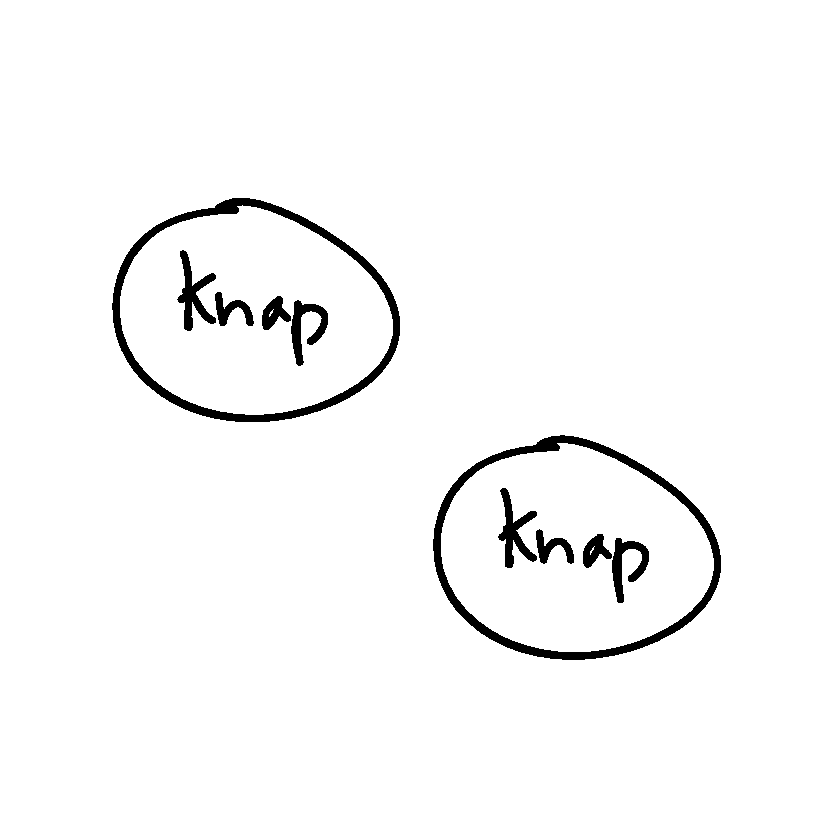
\includegraphics[scale=0.31]{img/sizeuden.pdf}\quad%
	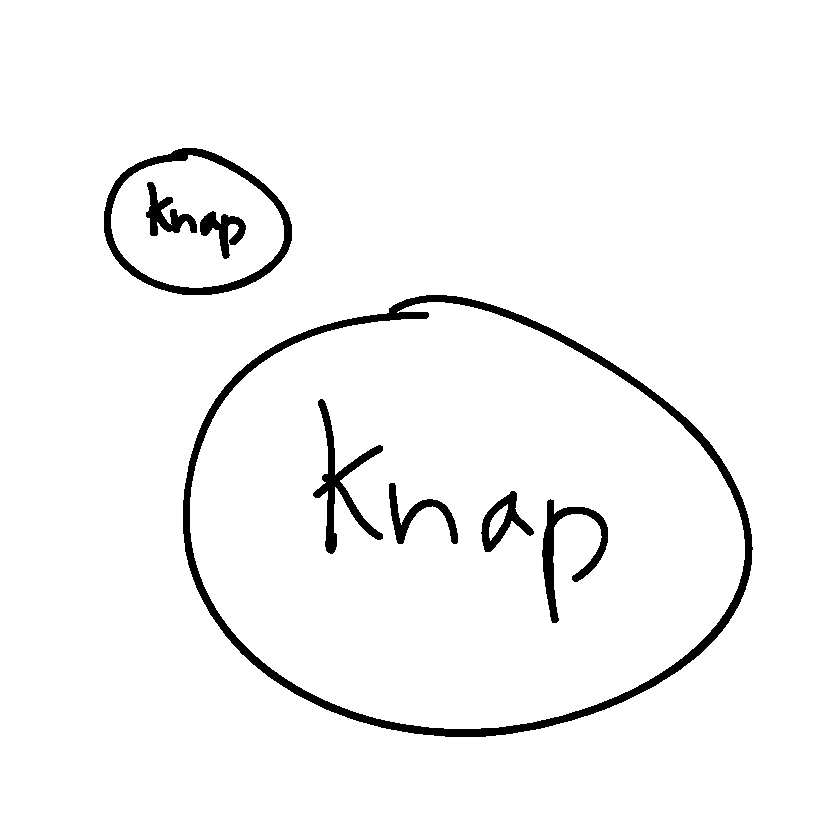
\includegraphics[scale=0.31]{img/sizemed.pdf}\quad%
	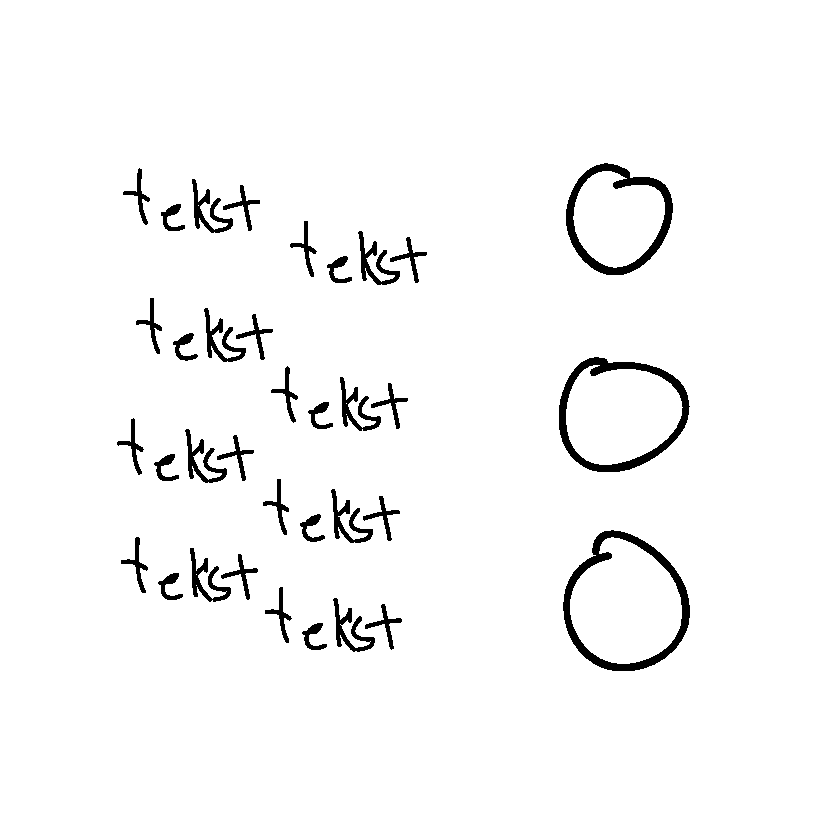
\includegraphics[scale=0.31]{img/boxinguden.pdf}\quad%
	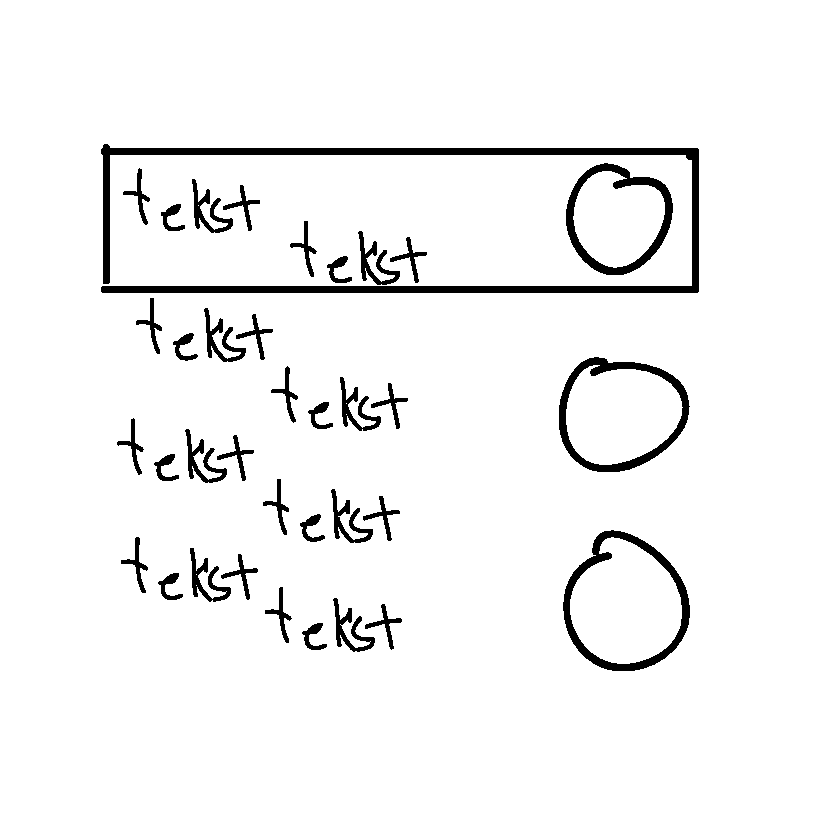
\includegraphics[scale=0.31]{img/boxingmed.pdf}
\end{frame}

\begin{frame}{Find principperne!}
	\centering
	\includegraphics[width=\linewidth]{img/bikester.jpg}
\end{frame}

\begin{frame}{Find principperne!}
	\centering
	\includegraphics[width=\linewidth]{img/currencyconvert.jpg}
\end{frame}

\begin{frame}{Opsummering}
	\begin{multicols}{2}
		\begin{itemize}
			\item Vi skal lære ting
			\item Engelsk, Matematik, Fysik
			\item Unity3D
			\item Android Studio
			\item X Code
			\item MIT App Inventor
			\item Scratch
			\item HTML5
			\item Agil
			\item Vandfald
			\item Design for mennesker
			\item Design for aktiviteter
			\item Design for kontekst
			\item Design nærhed
			\item Design mønstre
			\item Design opstilling
			\item Design kontrast
			\item Design størrelse
			\item Design adskillelse
		\end{itemize}
	\end{multicols}
\end{frame}
\section{Sketching \& Prototyping}

\begin{frame}{Ideation}
		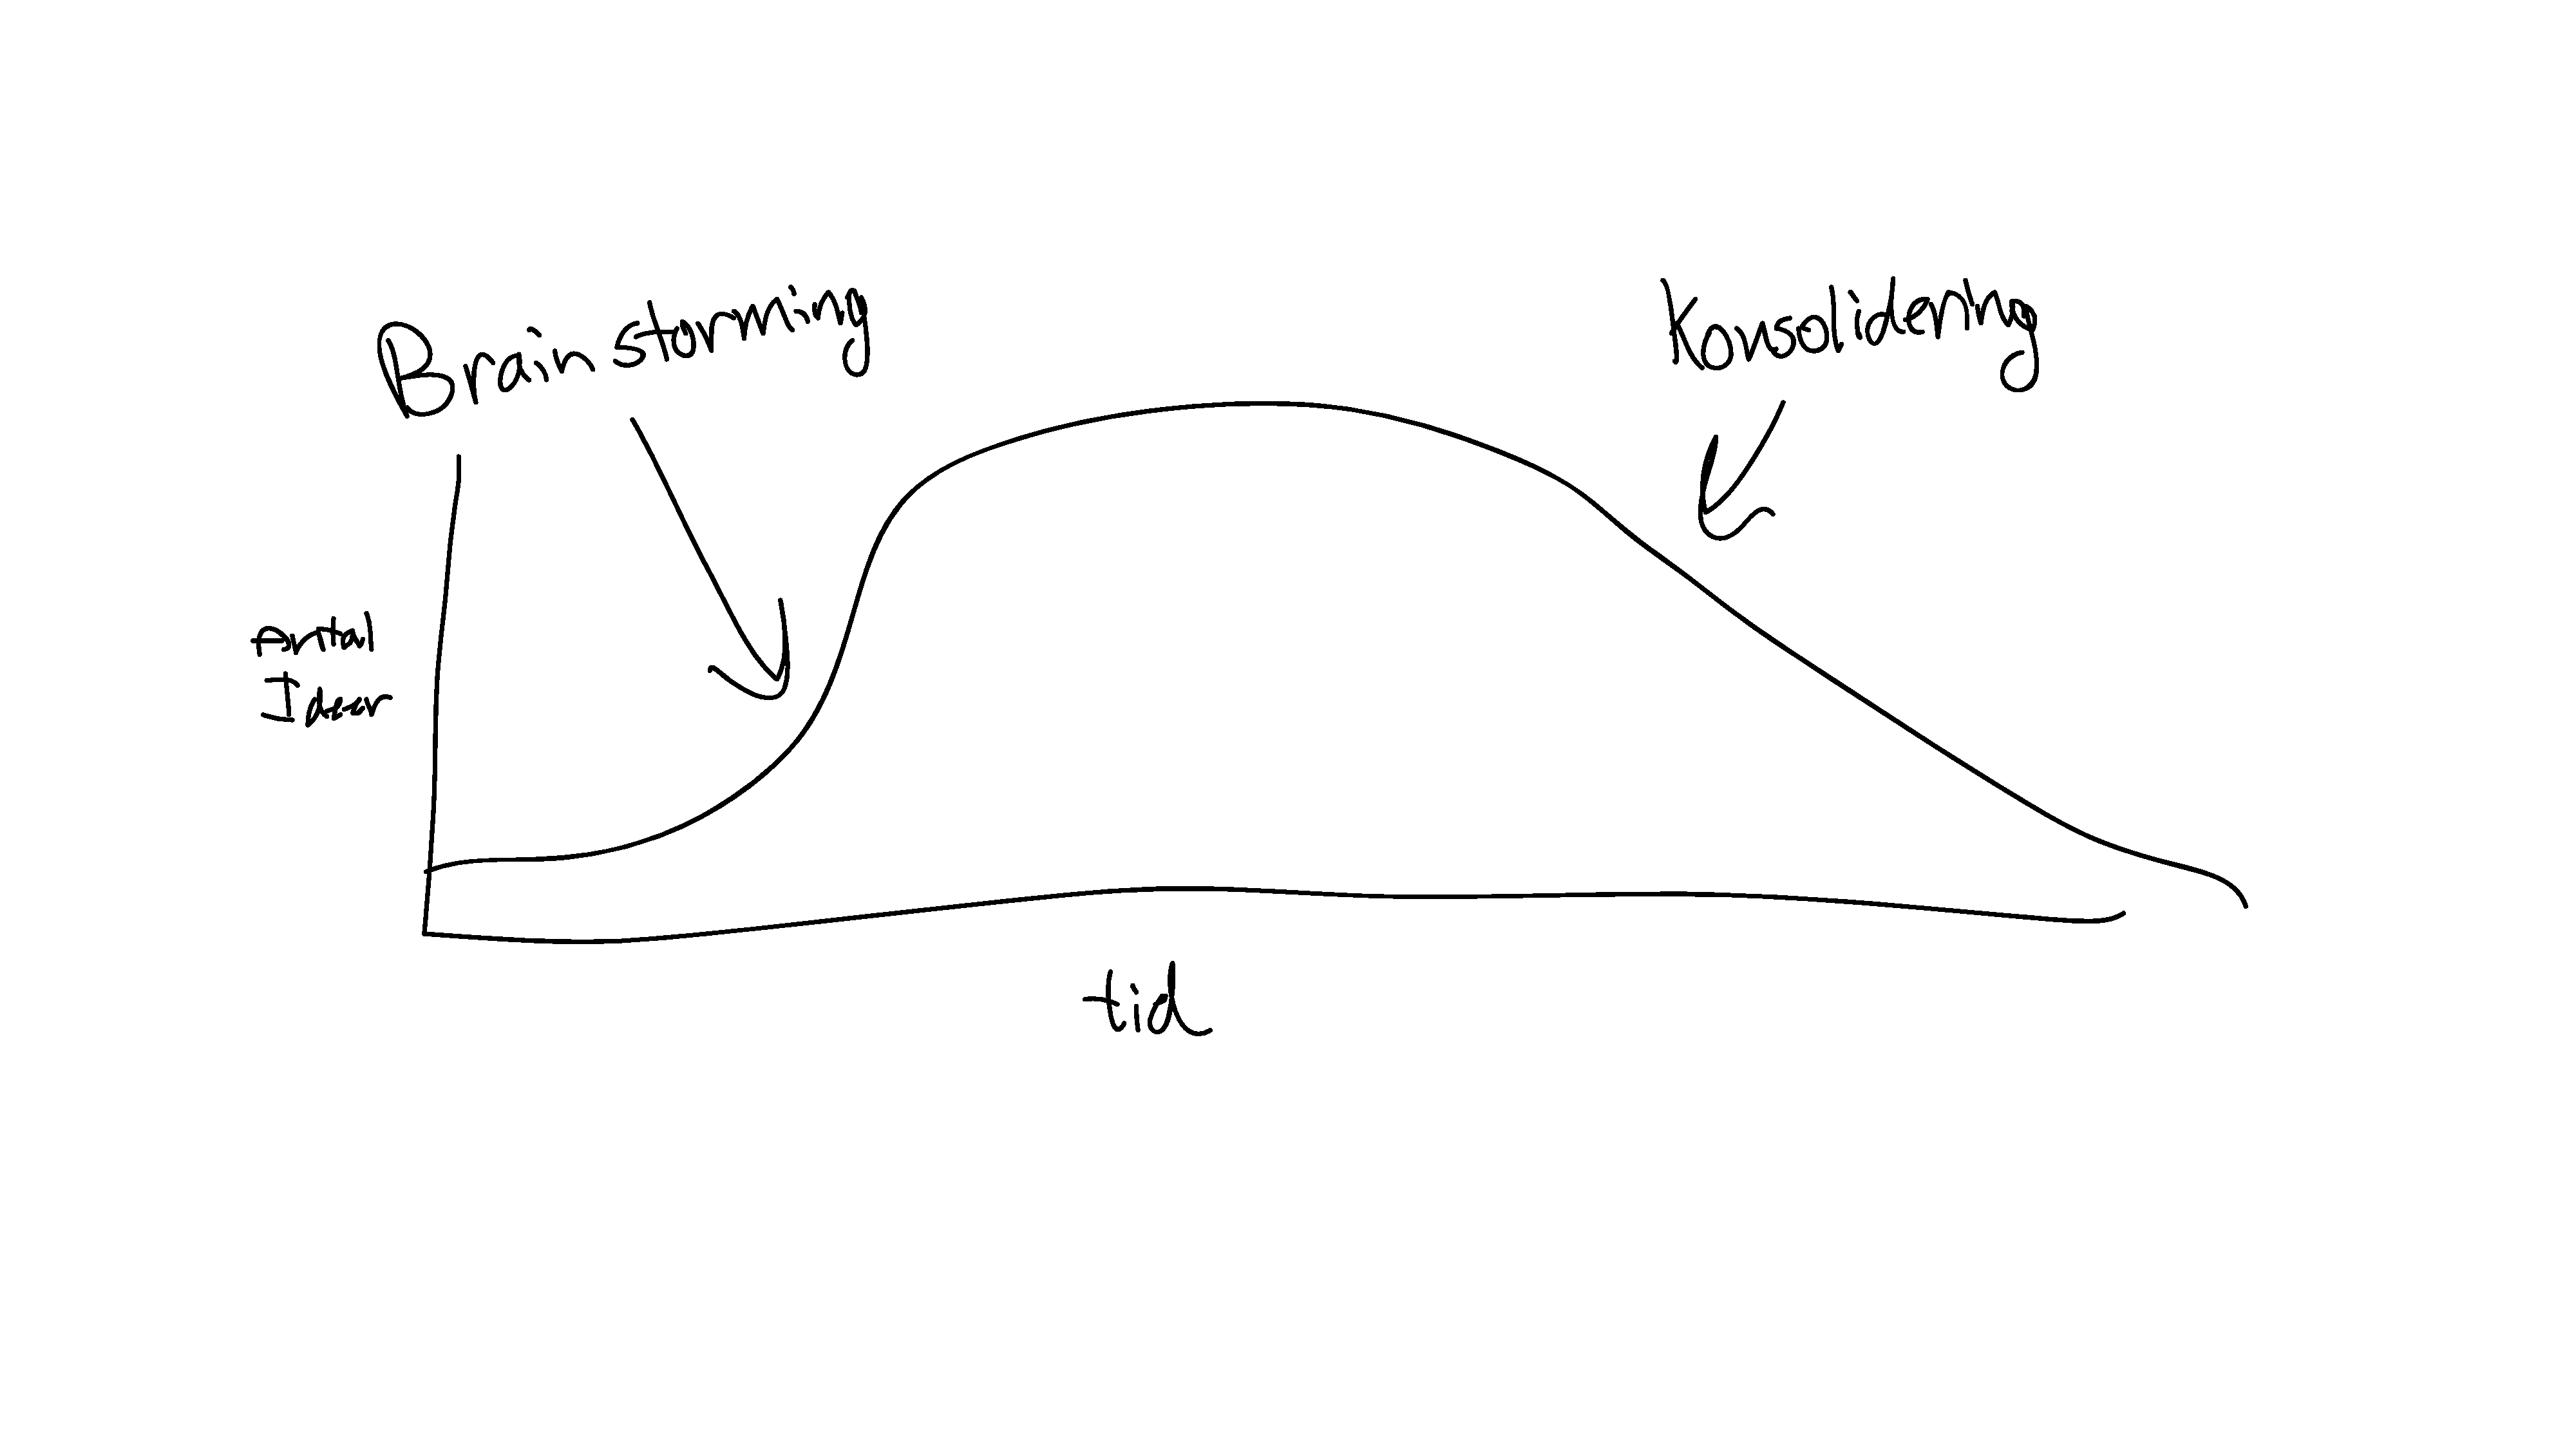
\includegraphics[scale=0.18]{img/ideation.pdf}
\end{frame}

\begin{frame}{Hvad er en sketch I}
	\centering
	\includegraphics[width=\linewidth]{img/operasketch.jpg}
\end{frame}

\begin{frame}{Hvad er en sketch II}
	\centering
	\includegraphics[width=\linewidth]{img/Sydney_opera_house.jpg}
\end{frame}

\begin{frame}{Hvad er prototyper I}
	\centering
	\includegraphics[width=\linewidth]{img/paperprotoyping.jpg}
\end{frame}

\begin{frame}{Hvad er prototyper II}
	\centering
	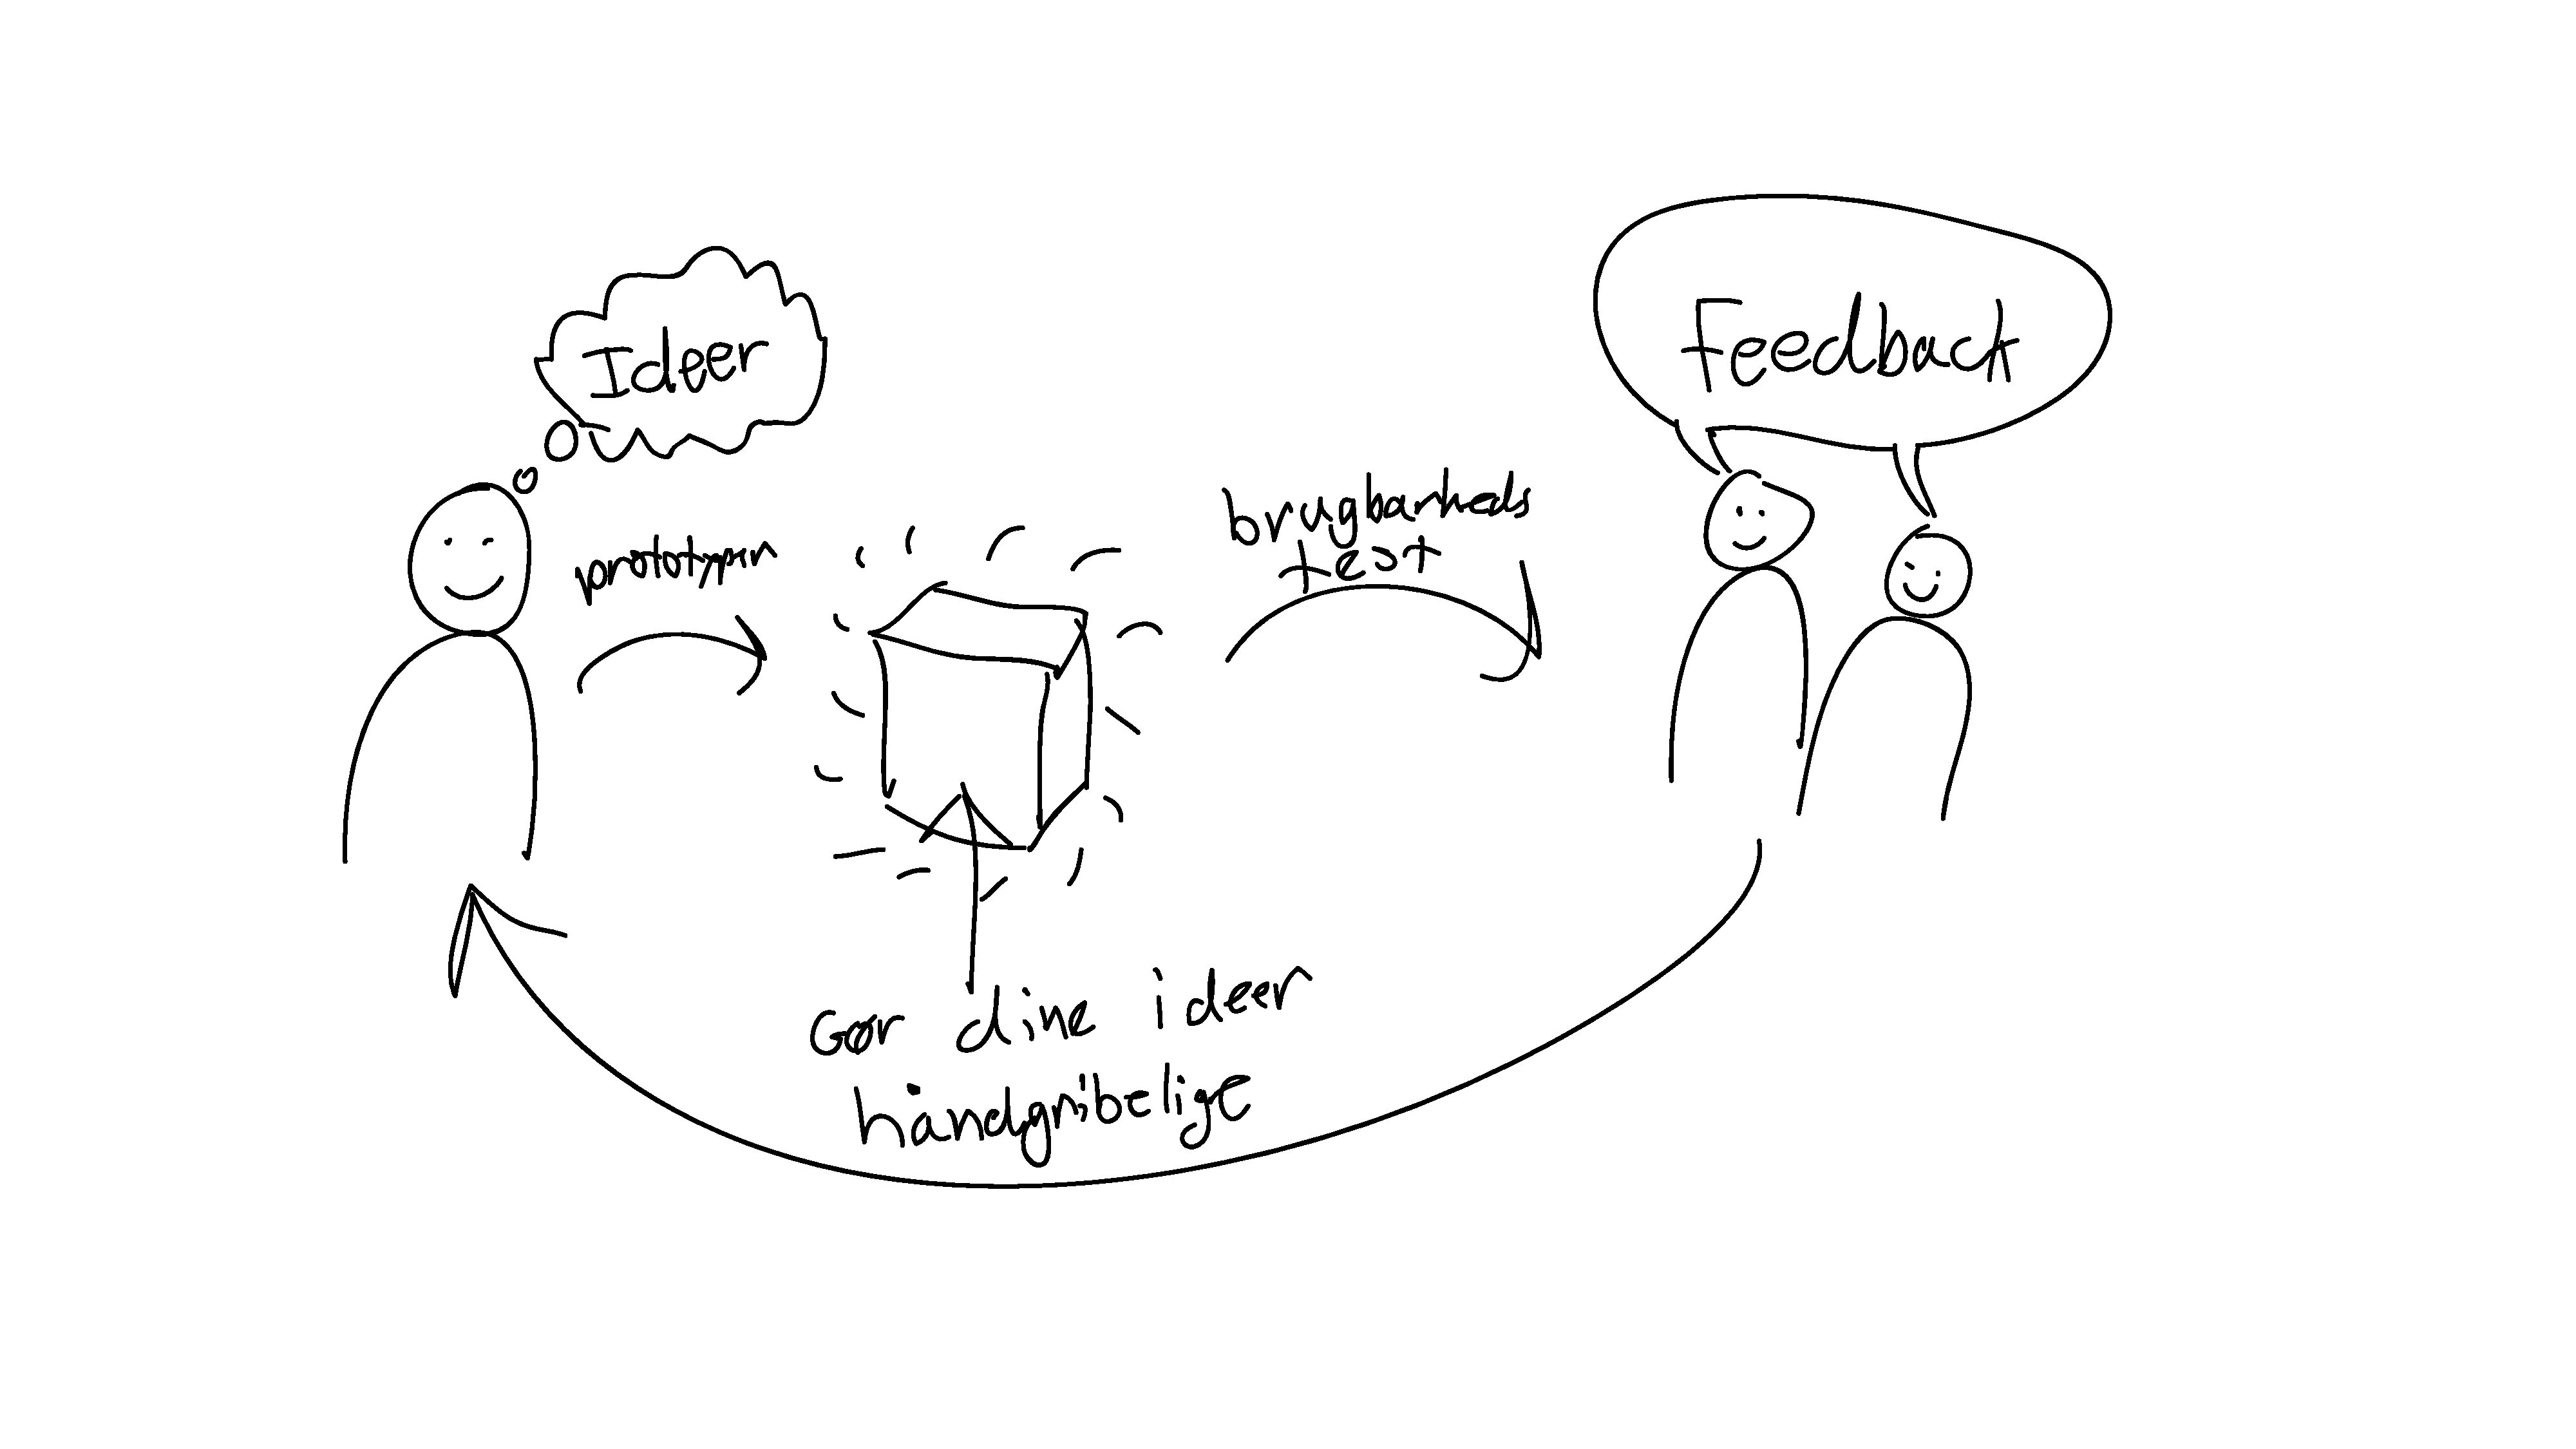
\includegraphics[scale=0.18]{img/prototypingloop.pdf}
\end{frame}

\begin{frame}{Sketch \& Prototype egenskaber}
\begin{center}
  \begin{tabular}{| l | l |}
    \hline
	\textbf{Sketch} & \textbf{Prototype} \\ \hline
    Hurtig & Knap så Hurtig\\ \hline
    Billig & Knap så Billig\\ \hline
    Talrige & Få \\ \hline
    Flertydige & Præcise \\ \hline
    Foreslår og udforsker & Uddyber \\ \hline
    Provokerer & Løser \\ \hline
    Giver spørgsmål & Giver svar \\ \hline
  \end{tabular}
\end{center}
\end{frame}

\plain{
Øvelse: 
Ide generation, Brainstorming.

Lav en masse sketches

f.eks. vejr app, 
 }

\begin{frame}{Prototyping Redskaber}
\centering
	\includegraphics[width=\linewidth]{img/tapeandtools.png}
\end{frame}

\begin{frame}{Prototyping Tricks}
\centering
	\includegraphics[width=\linewidth]{img/desktopsketch.png}
\end{frame}

\begin{frame}{Prototyping Tricks}
\centering
	\includegraphics[width=\linewidth]{img/pagessketch.png}
\end{frame}

\begin{frame}{Prototyping Tricks}
\centering
	\includegraphics[width=\linewidth]{img/sketchtricks.png}
\end{frame}

\begin{frame}{Prototyping Tricks}
\centering
	\includegraphics[width=\linewidth]{img/dropdown.png}
\end{frame}

\begin{frame}{Prototyping Tricks}
\centering
	\includegraphics[width=\linewidth]{img/expandablelists.png}
\end{frame}

\plain{
Øvelse:

Lav en prototype
 
 }


\end{document}
